\chapter{Chromatine en epigenetica}\label{ch:b3:chromatin-epigenetics}

Twee muizen uit hetzelfde nest, genetisch identiek tot aan de laatste
base, zitten naast elkaar: de ene is slank en bruin, de andere dik en
geel, en zij zal diabetes krijgen. Een lapjeskat draagt oranje en
zwarte vlekken hoewel elke cel van haar huid dezelfde twee
X-chromosomen bevat. Een kind erft hetzelfde ontbrekende stuk van
chromosoom 15 als een ander kind, en de een heeft het syndroom van
Prader--Willi terwijl de ander het syndroom van Angelman heeft --- het
verschil is alleen van welke ouder de deletie kwam. Niets hiervan
staat in de DNA-sequentie geschreven. Het staat er \emph{op}
geschreven: in de manier waarop twee meter DNA in een kern van tien
micrometer doorsnede wordt gepakt, in de kleine chemische groepen aan
de pakkingseiwitten en aan de cytosines zelf, en in de machinerie die
die merktekens van een cel naar haar dochters kopieert. Dit hoofdstuk
gaat over die tweede informatielaag, haar moleculaire dragers en de
eerlijke grenzen aan wat zij kan onthouden.

\section{Chromatine: DNA op een klos}

\begin{definition}[Nucleosoom en chromatine]\label{def:b3:chromatin-epigenetics:nucleosome}
\index{nucleosoom}\index{chromatine}\index{histon}\index{euchromatine}\index{heterochromatine}
\emph{Chromatine} is het complex van DNA met eiwitten waarin het
genoom in een eukaryote kern bestaat. De herhalende eenheid is het
\emph{nucleosoom}: \qty{147}{bp} DNA gewonden in $1.65$ linksdraaiende
slagen om een octameer van \emph{histonen} --- van elk van de kleine,
zeer basische eiwitten H2A, H2B, H3 en H4 twee kopieën --- gevolgd
door een \emph{linker} van \qtyrange{20}{60}{bp} naar het volgende
nucleosoom. Een vijfde histon, H1, bindt de linker waar die de kern
binnengaat en verlaat en helpt de kralen tegen elkaar aan te pakken.
Elk kernhiston draagt een ongestructureerde aminoterminale
\emph{staart} van zo'n \numrange{20}{40} residuen die uit het deeltje
steekt. Chromatine dat licht kleurt, los gepakt is en wordt
getranscribeerd heet \emph{euchromatine}; dicht gepakt, laat
replicerend en grotendeels zwijgend chromatine, bij centromeren,
telomeren en herhaalde sequenties, heet \emph{heterochromatine}.
\end{definition}

\begin{proof}[Bewijsmateriaal]
Hewish en Burgoyne (1973) verteerden rattenleverkernen met een
endogeen nuclease en vonden dat het DNA er niet als een veeg uit kwam
maar als een ladder van fragmenten met lengtes die veelvouden waren
van ongeveer \qty{200}{bp}: het DNA was op regelmatige afstanden
beschermd en werd alleen ertussen geknipt. Kornberg (1974) toonde aan
dat de beschermde eenheid een deeltje van acht \omterm{def:b3:chromatin-epigenetics:nucleosome}{histonen} met ongeveer
\qty{200}{bp} was, en elektronenmicroscopische opnamen van voorzichtig
uitgespreid \omterm{def:b3:chromatin-epigenetics:nucleosome}{chromatine} lieten de ``kralen aan een snoer'' zien. Luger
en collega's (1997) losten de kristalstructuur van het kerndeeltje op
bij \qty{2.8}{\angstrom}: \qty{147}{bp}, een octameer met de staarten
tussen de DNA-windingen door naar buiten.
\end{proof}

\begin{omfigure}
\begin{tikzpicture}[every node/.style={font=\scriptsize}, >=stealth]
  % beads on a string
  \foreach \x/\y in {0/0, 2.2/0.5, 4.4/0, 6.6/0.5, 8.8/0} {
    \fill[omDef!30] (\x,\y) circle (0.42);
    \draw[very thick, omThm!70!black] (\x,\y) circle (0.5);
  }
  \draw[very thick, omThm!70!black] (-1.1,-0.1) -- (0-0.47,-0.17);
  \draw[very thick, omThm!70!black] (0.47,-0.17) -- (2.2-0.47,0.33);
  \draw[very thick, omThm!70!black] (2.67,0.33) -- (4.4-0.47,-0.17);
  \draw[very thick, omThm!70!black] (4.87,-0.17) -- (6.6-0.47,0.33);
  \draw[very thick, omThm!70!black] (7.07,0.33) -- (8.8-0.47,-0.17);
  \draw[very thick, omThm!70!black] (9.27,-0.17) -- (10.4,-0.1);
  % tails
  \foreach \x/\y in {0/0, 4.4/0, 8.8/0} { \draw[omProp, thick] (\x,\y+0.5) .. controls (\x-0.2,\y+0.9) .. (\x+0.1,\y+1.15); \draw[omProp, thick] (\x,\y-0.5) .. controls (\x+0.2,\y-0.9) .. (\x-0.1,\y-1.15); }
  \foreach \x/\y in {2.2/0.5, 6.6/0.5} { \draw[omProp, thick] (\x,\y+0.5) .. controls (\x-0.2,\y+0.9) .. (\x+0.1,\y+1.15); }
  % H1
  \fill[omMeth!70!black] (1.55,0.05) circle (0.12); \fill[omMeth!70!black] (5.95,0.05) circle (0.12);
  % labels
  \node[above, align=center] at (2.2,1.75) {histonstaarten\\(acetylering, methylering)};
  \node[below, align=center] at (4.4,-1.35) {kerndeeltje: octameer\\$+$ \qty{147}{bp}, $1.65$ slagen};
  \node[below, align=center] at (7.7,-0.55) {linker-DNA\\\qtyrange{20}{60}{bp}};
  \node[below] at (5.95,-0.1) {H1};
  \draw[<->] (-0.5,-2.2) -- (2.2-0.5,-2.2) node[midway, below] {herhaling $\approx \qty{200}{bp}$, \qty{11}{nm}};
  \draw[gray] (-0.5,-1.95) -- (-0.5,-2.35); \draw[gray] (1.7,-1.95) -- (1.7,-2.35);
\end{tikzpicture}

{\small De \qty{10}{nm}-vezel: nucleosoomkernen (blauw) op één
doorlopend DNA (rood), elke kraal een histonoctameer met zijn staarten
(oranje) naar buiten, linkerhiston H1 (groen) op het in- en
uittredepunt. Ongeveer zes \omterm{def:b3:chromatin-epigenetics:nucleosome}{nucleosomen} beslaan de lengte die
\qty{1200}{bp} naakt DNA zou innemen.}
\end{omfigure}

\begin{omfigure}
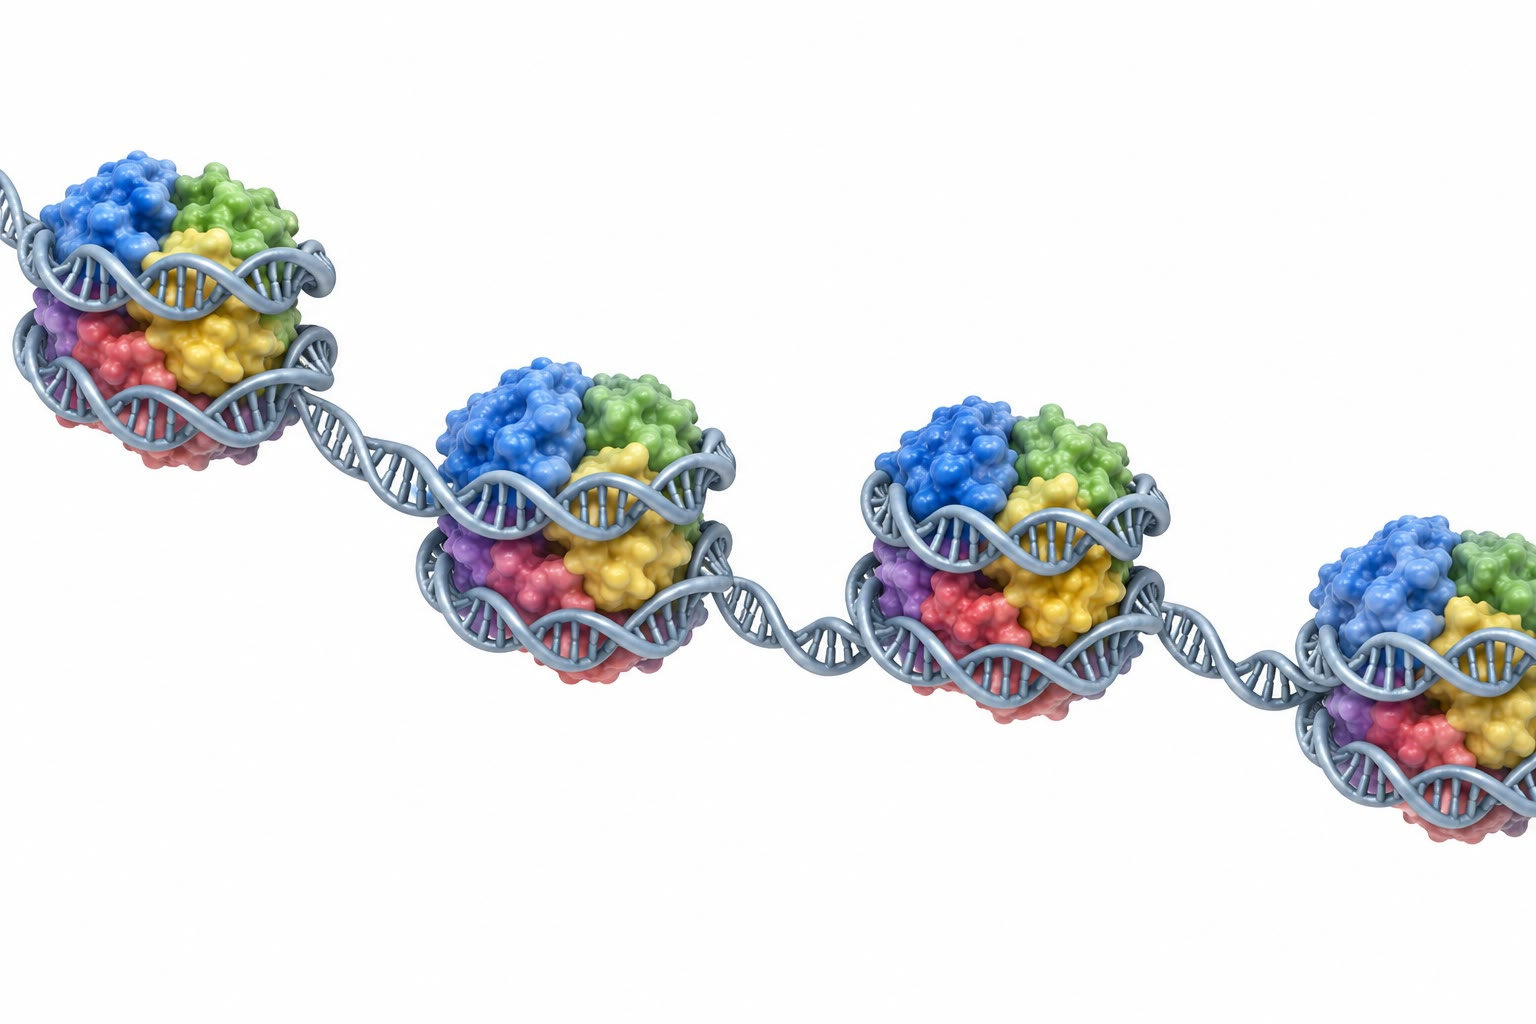
\includegraphics[width=0.6\linewidth]{images/book5/ai/b5-01-nucleosomes.jpg}

{\small \omterm{def:b3:chromatin-epigenetics:nucleosome}{Chromatine} op moleculaire schaal: de dubbele helix gewonden om
opeenvolgende histonkernen, de ``kralen aan een snoer'' die de
nucleaseladder aan het licht bracht.}
\end{omfigure}

\begin{proposition}[Niveaus van compactie]\label{prop:b3:chromatin-epigenetics:compaction}
\index{pakkingsgraad}\index{chromatinelus}\index{topologisch associërend domein}
De \emph{\omterm{prop:b3:chromatin-epigenetics:compaction}{pakkingsgraad}} van een chromatinestructuur is de lengte van
het DNA dat zij bevat gedeeld door de lengte van de structuur. Het
opwinden tot de \qty{10}{nm}-vezel geeft een graad van ongeveer $6$:
de \qty{68}{nm} van een herhaling van \qty{200}{bp} wordt samengeperst
tot één kraal van \qty{11}{nm}. In de interfasekern is de vezel niet
opgewonden tot een regelmatige dikkere vezel, zoals leerboeken haar
lang tekenden, maar gevouwen tot \emph{lussen} van tientallen tot
honderden kilobasen die aan hun voet worden vastgehouden door
ringvormige cohesinecomplexen en door het DNA-bindende eiwit CTCF; de
lussen groeperen zich tot \emph{topologisch associërende domeinen}
(TAD's) van ongeveer een megabase, waarbinnen een gen zijn regulatoren
veel vaker ontmoet dan wat dan ook daarbuiten. Een mitotisch
chromosoom, de meest compacte toestand, heeft een \omterm{prop:b3:chromatin-epigenetics:compaction}{pakkingsgraad} van
bijna \num{10000}: de \qty{4}{cm} DNA van een gemiddeld menselijk
chromosoom is gevouwen tot een staafje van \qty{4}{\micro m} lang.
\end{proposition}

\begin{example}[Twee meter in tien micrometer]\label{ex:b3:chromatin-epigenetics:two-metres}
Een menselijke diploïde kern bevat $6.4\times 10^{9}$ basenparen. Bij
\qty{0.34}{nm} per basenpaar is dat \qty{2.2}{m} dubbele helix, in een
kern van ongeveer \qty{10}{\micro m} doorsnede. Zij wordt gepakt in
$6.4\times 10^{9}/200 \approx 3.2\times 10^{7}$ \omterm{def:b3:chromatin-epigenetics:nucleosome}{nucleosomen}, die elk
ongeveer \qty{108}{kDa} \omterm{def:b3:chromatin-epigenetics:nucleosome}{histon} dragen tegenover \qty{96}{kDa} DNA
(\qty{147}{bp} à \qty{650}{Da} per paar): de kern bevat naar massa
ruwweg evenveel \omterm{def:b3:chromatin-epigenetics:nucleosome}{histon} als DNA. Het DNA zelf, opgevat als een cilinder
van \qty{2}{nm} doorsnede, heeft een volume van slechts ongeveer
\qty{7}{\micro m^3}, zo'n \qty{1}{\%} van een bolvormige kern met
straal \qty{5}{\micro m}; het pakkingsprobleem is er een van
verknoping en toegang, niet van ruimte.
\end{example}

\section{De histoncode}

\begin{definition}[Histonmodificaties]\label{def:b3:chromatin-epigenetics:histone-code}
\index{histoncode}\index{acetylering}\index{histonmethylering}\index{schrijver}\index{lezer}\index{wisser}
De residuen van de histonstaarten worden covalent gemodificeerd:
\emph{acetylering} van lysines (die hun positieve lading neutraliseert
en de greep op het DNA losser maakt), \emph{methylering} van lysines
en arginines (één, twee of drie methylgroepen, zonder verandering van
lading), fosforylering van serines, ubiquitinering van lysines. Een
modificatie wordt genoemd naar \omterm{def:b3:chromatin-epigenetics:nucleosome}{histon}, residu en groep: H3K4me3 is
\omterm{def:b3:chromatin-epigenetics:nucleosome}{histon} H3, lysine 4, getrimethyleerd; H3K27ac is H3 lysine 27
geacetyleerd. De \emph{histoncode} is het verband tussen combinaties
van merktekens en de toestand van het onderliggende gen: H3K4me3 en
H3K27ac op actieve promotoren en enhancers, H3K36me3 langs
getranscribeerde genlichamen, H3K9me3 op constitutief
\omterm{def:b3:chromatin-epigenetics:nucleosome}{heterochromatine}, H3K27me3 op genen die tijdens de ontwikkeling zijn
uitgeschakeld. Enzymen die een merkteken aanbrengen zijn
\emph{schrijvers} (histonacetyltransferasen, HAT's; methyltransferasen),
enzymen die het verwijderen zijn \emph{wissers} (histondeacetylasen,
HDAC's; demethylasen), en eiwitten die een merkteken binden en erop
reageren zijn \emph{lezers}: een \emph{bromodomein} bindt
acetyllysine, een \emph{chromodomein} methyllysine.
\end{definition}

\begin{proposition}[Merktekens worden gelezen, niet slechts gevoeld]\label{prop:b3:chromatin-epigenetics:readers}
\index{HP1}\index{Polycomb}\index{PRC2}\index{Trithorax}
\omterm{def:b3:chromatin-epigenetics:histone-code}{Acetylering} werkt deels langs elektrostatische weg --- een
geacetyleerde staart houdt zijn DNA minder stevig vast en de vezel
opent zich --- maar de meeste merktekens werken door \omterm{def:b3:chromatin-epigenetics:histone-code}{lezers} aan te
trekken. H3K9me3 wordt gebonden door het chromodomein van het
\emph{heterochromatine-eiwit HP1}, dat dimeriseert, naburige
\omterm{def:b3:chromatin-epigenetics:nucleosome}{nucleosomen} overbrugt en juist het methyltransferase (SUV39H)
aantrekt dat H3K9me3 op het volgende \omterm{def:b3:chromatin-epigenetics:nucleosome}{nucleosoom} schrijft: het
merkteken breidt zich langs de vezel uit tot het een grens bereikt, en
comprimeert wat het bedekt. H3K27me3 wordt geschreven door
\emph{Polycomb repressive complex 2} (PRC2, katalytische subeenheid
EZH2), gelezen door PRC1, dat H2A ubiquitineert en de vezel
comprimeert, en het complex wordt zelf gestimuleerd door het merkteken
dat het maakt; de \emph{Trithorax}-groep van eiwitten schrijft het
tegengestelde H3K4me3 en houdt de ontwikkelingsgenen van een bepaald
celtype aan. Elke zulke lus --- een \omterm{def:b3:chromatin-epigenetics:histone-code}{lezer} trekt een \omterm{def:b3:chromatin-epigenetics:histone-code}{schrijver} aan --- is
een positieve terugkoppeling die een toestand zichzelf laat handhaven
zodra hij gevestigd is, en dat is wat een erfelijk merkteken nodig heeft.
\end{proposition}

\begin{omfigure}
\begin{tikzpicture}[every node/.style={font=\scriptsize}, >=stealth]
  % nucleosomes with tails
  \foreach \x in {0,2,4,6} { \draw[thick, omDef, fill=omDef!20] (\x,0) circle (0.45); \draw[omProp, thick] (\x,0.45) -- (\x,1.15); }
  % marks
  \fill[omThm] (2,1.15) circle (0.11); \fill[omThm] (4,1.15) circle (0.11);
  \fill[omMeth!80!black] (0,1.15) circle (0.11);
  \node[left] at (-0.5,1.15) {ac};
  \node[right, align=left] at (6.15,1.15) {me3};
  % HP1 reader
  \draw[thick, fill=omExo!30] (2.6,1.7) ellipse (0.5 and 0.25); \node at (2.6,1.7) {lezer};
  \draw[thick, fill=omExo!30] (4.2,2.35) ellipse (0.55 and 0.25); \node at (4.2,2.35) {schrijver};
  \draw[->, thick] (2.9,1.9) -- (3.75,2.2);
  \draw[->, thick, omThm] (4.6,2.15) .. controls (5.6,2.0) and (6.1,1.8) .. (6.05,1.3);
  \node[right, align=left, font=\scriptsize] at (6.6,2.0) {breidt uit naar het\\volgende nucleosoom};
  \draw[->, thick, gray] (2.2,1.3) -- (2.45,1.5);
  % eraser
  \draw[thick, fill=omExo!30] (0.6,2.2) ellipse (0.5 and 0.25); \node at (0.6,2.2) {wisser};
  \draw[->, thick, omMeth!80!black] (0.3,2.0) -- (0.05,1.35);
  % DNA
  \draw[very thick, omThm!70!black] (-0.9,-0.3) -- (-0.45,-0.05) (0.45,-0.05) -- (1.55,-0.05) (2.45,-0.05) -- (3.55,-0.05) (4.45,-0.05) -- (5.55,-0.05) (6.45,-0.05) -- (7.2,-0.3);
  \node[below, align=center] at (0,-0.6) {open: acetylgroep\\haalt een lading weg};
  \node[below, align=center] at (5,-0.6) {dicht: HP1 leest H3K9me3\\en trekt het K9-methylase aan};
\end{tikzpicture}

{\small De logica van \omterm{def:b3:chromatin-epigenetics:histone-code}{schrijver}, \omterm{def:b3:chromatin-epigenetics:histone-code}{lezer} en \omterm{def:b3:chromatin-epigenetics:histone-code}{wisser}. Een \omterm{def:b3:chromatin-epigenetics:histone-code}{lezer} die op een
merkteken van het ene \omterm{def:b3:chromatin-epigenetics:nucleosome}{nucleosoom} zit, trekt de \omterm{def:b3:chromatin-epigenetics:histone-code}{schrijver} aan die
hetzelfde merkteken op het volgende zet, zodat de toestand zich
uitbreidt en zichzelf kopieert; \omterm{def:b3:chromatin-epigenetics:histone-code}{wissers} werken ertegen. Acetylgroepen
(groen) openen de vezel; H3K9me3 (rood) sluit haar.}
\end{omfigure}

\begin{method}[Chromatine-immunoprecipitatie (ChIP)]\label{met:b3:chromatin-epigenetics:chip}
\index{ChIP}\index{chromatine-immunoprecipitatie}
Om in kaart te brengen waar een merkteken of een eiwit op het genoom
zit: (1) verknoop eiwitten en DNA in levende cellen met formaldehyde;
(2) breek het \omterm{def:b3:chromatin-epigenetics:nucleosome}{chromatine} in fragmenten van enkele honderden
basenparen; (3) sla de fragmenten neer met een aan kralen gebonden
antilichaam tegen het merkteken (bijvoorbeeld H3K27me3); (4) maak de
verknopingen ongedaan en zuiver het DNA; (5) sequenceer het (ChIP-seq)
en tel de reads langs het genoom: de pieken zijn de plaatsen waar het
merkteken zat. Een controle van ingangs-DNA zonder antilichaam bepaalt
de achtergrond. De resolutie is die van de fragmenten, ongeveer één
\omterm{def:b3:chromatin-epigenetics:nucleosome}{nucleosoom}.
\end{method}

\begin{remark}[Code of correlatie]\label{rem:b3:chromatin-epigenetics:code}
Het woord ``code'' zegt te veel. Veel merktekens zijn eerder gevolgen
van transcriptie dan oorzaken ervan (H3K36me3 wordt neergelegd door
een methyltransferase dat met het polymerase meerijdt), en het
weghalen van een \omterm{def:b3:chromatin-epigenetics:histone-code}{schrijver} verandert de expressie vaak veel minder dan
de verdeling van het merkteken doet vermoeden. Wat wel vaststaat, is
dat enkele merktekens --- H3K9me3, H3K27me3 en de \omterm{def:b3:chromatin-epigenetics:methylation}{DNA-methylering}
hieronder --- een zelfvoortplantende uitschakeling dragen die het
signaal overleeft dat haar heeft ingesteld.
\end{remark}

\section{DNA-methylering en het kopiëren van een merkteken}

\begin{definition}[DNA-methylering]\label{def:b3:chromatin-epigenetics:methylation}
\index{DNA-methylering}\index{CpG}\index{CpG-eiland}\index{DNMT1}\index{onderhoudsmethylering}\index{de-novomethylering}
Bij gewervelden wordt vrijwel alleen in het dinucleotide \emph{CpG}
(een C gevolgd door een G op dezelfde streng) een methylgroep aan
koolstof 5 van cytosine gehangen, een sequentie die haar eigen
complement is, zodat een gemethyleerd CpG normaal op beide strengen
gemethyleerd is. Zo'n \qtyrange{70}{80}{\%} van de CpG's van een
menselijke cel is gemethyleerd, en gemethyleerde promotoren zwijgen:
de methylgroepen worden gelezen door methyl-CpG-bindende eiwitten
(MeCP2, MBD1--4) die HDAC's en H3K9-methylasen aantrekken, en zij
blokkeren verscheidene transcriptiefactoren rechtstreeks. De
uitzonderingen zijn de \emph{CpG-eilanden}, stukken van ongeveer een
kilobase, rijk aan G en C en aan CpG, die bij de promotoren van de
meeste huishoudgenen liggen en in normale cellen ongemethyleerd
blijven. De methylgroep wordt geschreven door
\emph{DNA-methyltransferasen}: DNMT3A en DNMT3B verzorgen de
\emph{de-novomethylering} van ongemethyleerde plaatsen, en
\emph{DNMT1}, dat een hemigemethyleerd CpG verkiest --- de ene streng
gemethyleerd, de andere niet --- verzorgt de
\emph{onderhoudsmethylering} achter de replicatievork. Verwijdering is
passief, door replicatie zonder onderhoud, of actief, door de
TET-enzymen, die 5-methylcytosine oxideren tot
5-hydroxymethylcytosine en verder, tot base-excisieherstel het door
een gewoon cytosine vervangt.
\end{definition}

\begin{example}[Waarom het genoom arm is aan CpG]\label{ex:b3:chromatin-epigenetics:cpg-deficit}
Het menselijk genoom is voor \qty{42}{\%} G$+$C, dus als de basen
onafhankelijk waren zou een \omterm{def:b3:chromatin-epigenetics:methylation}{CpG} voorkomen met frequentie
$0.21\times 0.21 \approx 0.044$, ongeveer $2.8\times 10^{8}$ keer in
het diploïde genoom. Het waargenomen aantal is ongeveer
$5.6\times 10^{7}$, een vijfde daarvan. De oorzaak is het merkteken
zelf: een gemethyleerd cytosine dat zijn aminogroep verliest wordt
thymine, een normale base die het herstel niet als fout kan herkennen,
terwijl een ongemethyleerd cytosine tot uracil deamineert, dat wordt
uitgesneden. In de loop van de evolutie zijn gemethyleerde \omterm{def:b3:chromatin-epigenetics:methylation}{CpG}'s tot
TpG en CpA gemuteerd, en alleen de ongemethyleerde eilanden hebben hun
\omterm{def:b3:chromatin-epigenetics:methylation}{CpG}'s behouden. Het merkteken heeft zijn handtekening in de sequentie
achtergelaten.
\end{example}

\begin{theorem}[Behoud van een methyleringstoestand door de delingen heen]\label{thm:b3:chromatin-epigenetics:maintenance}
\index{epigenetisch geheugen}\index{markovketen!methylering}
Beschouw één CpG-plaats, gevolgd langs een lijn van cellen. Bij elke
deling wordt het cytosine van de nieuwe streng gemethyleerd met kans
$\mu$ als het cytosine van de matrijsstreng gemethyleerd is
(onderhoudsefficiëntie) en met kans $\delta$ als dat niet zo is
(de-novosnelheid). Zij $p_{n}$ de kans dat de plaats na $n$ delingen
gemethyleerd is. Dan geldt
\[
p_{n+1} = \mu\, p_{n} + \delta\,(1 - p_{n}),
\qquad
p_{n} = p^{*} + (p_{0} - p^{*})\,(\mu - \delta)^{n},
\qquad
p^{*} = \frac{\delta}{1 - \mu + \delta}.
\]
Elke plaats drijft naar hetzelfde evenwicht $p^{*}$, wat haar
begintoestand ook is, en het geheugen van de begintoestand vervalt
meetkundig met verhouding $\mu - \delta$. Een merkteken wordt ongeveer
$1/(1 - \mu + \delta)$ delingen lang onthouden; trouw geheugen van een
\emph{verschil} tussen plaatsen vereist daarom dat $\mu$ zeer dicht bij
$1$ ligt en $\delta$ zeer dicht bij $0$, of een terugkoppeling die
$\mu$ en $\delta$ van de toestand van de omgeving laat afhangen.
\end{theorem}
\begin{proof}
De recursie is de wet van de totale kans over de twee toestanden van
de matrijs. Het vaste punt lost $p^{*} = \mu p^{*} + \delta(1 -
p^{*})$ op, wat $p^{*}(1 - \mu + \delta) = \delta$ geeft. Trekt men de
vergelijking van het vaste punt van de recursie af, dan is
$p_{n+1} - p^{*} = (\mu -
\delta)(p_{n} - p^{*})$, wat itereert tot de gesloten vorm. Omdat
$0 \le \delta \le \mu \le 1$ ligt de verhouding $\mu - \delta$ in $[0,1]$
en krimpt de afwijking; zij halveert elke $\ln 2 / (-\ln(\mu -
\delta)) \approx \ln 2/(1 - \mu + \delta)$ delingen wanneer $\mu -
\delta$ dicht bij $1$ ligt.
\end{proof}

\begin{example}[Getallen]\label{ex:b3:chromatin-epigenetics:maintenance-numbers}
Gemeten waarden voor zoogdiercellen zijn $\mu \approx 0.99$ en
$\delta \approx 0.02$ per deling op een gewoon \omterm{def:b3:chromatin-epigenetics:methylation}{CpG}. Dan is $p^{*} =
0.02/0.03 \approx 0.67$, dicht bij de genoombrede gemethyleerde
fractie, en $\mu - \delta = 0.97$: een volledig gemethyleerde plaats
die alleen aan de machinerie wordt overgelaten zou na $\ln 2 /
0.03 \approx 23$ delingen halverwege terug zijn naar het gemiddelde.
Een uitgeschakelde promotor die de honderden delingen van een leven
lang blijft zwijgen heeft daarom meer nodig dan \omterm{def:b3:chromatin-epigenetics:methylation}{DNMT1}: de
methyl-CpG-lezers trekken H3K9-methylering aan en de H3K9-lezers
trekken DNMT3 aan, zodat een dicht eiland van merktekens zijn eigen
$\mu$ naar $1$ opdrijft en de naburige $\delta$ naar $0$ verlaagt.
Omgekeerd verliest een cel die \omterm{def:b3:chromatin-epigenetics:methylation}{DNMT1} kwijtraakt het merkteken passief:
met $\mu = \delta = 0$ halveert de fractie gemethyleerde strengen bij
elke deling.
\end{example}

\begin{omfigure}
\begin{tikzpicture}[every node/.style={font=\scriptsize}, >=stealth]
  % left: replication scheme
  \begin{scope}
    \draw[very thick, omThm!70!black] (0,1.2) -- (2.4,1.2); \draw[very thick, omThm!70!black] (0,0.9) -- (2.4,0.9);
    \foreach \x in {0.5,1.2,1.9} { \fill[omDef] (\x,1.2) circle (0.09); \fill[omDef] (\x,0.9) circle (0.09); }
    \node[above] at (1.2,1.3) {ouderlijk: beide strengen gemethyleerd};
    \draw[->, thick] (1.2,0.75) -- (1.2,0.15) node[midway, right] {replicatie};
    \draw[very thick, omThm!70!black] (0,-0.1) -- (2.4,-0.1); \draw[very thick, gray] (0,-0.4) -- (2.4,-0.4);
    \foreach \x in {0.5,1.2,1.9} { \fill[omDef] (\x,-0.1) circle (0.09); \draw[omDef] (\x,-0.4) circle (0.09); }
    \node[left] at (-0.1,-0.25) {hemigemethyleerd};
    \draw[->, thick] (1.2,-0.85) -- (1.2,-1.45) node[midway, right, align=left] {DNMT1, kans $\mu$\\per plaats};
    \draw[very thick, omThm!70!black] (0,-1.7) -- (2.4,-1.7); \draw[very thick, gray] (0,-2.0) -- (2.4,-2.0);
    \foreach \x in {0.5,1.9} { \fill[omDef] (\x,-1.7) circle (0.09); \fill[omDef] (\x,-2.0) circle (0.09); }
    \fill[omDef] (1.2,-1.7) circle (0.09); \draw[omDef] (1.2,-2.0) circle (0.09);
    \node[below, align=center] at (1.2,-2.1) {hersteld, één plaats gemist:\\de nieuwe streng van de dochter};
  \end{scope}
  % right: decay plot
  \begin{scope}[xshift=5.0cm, yshift=-2.3cm]
  \begin{axis}[
    width=6.6cm, height=4.6cm, axis lines=left,
    xmin=0, xmax=100, ymin=0, ymax=1.05,
    xlabel={delingen $n$},
    xlabel style={font=\scriptsize, at={(axis description cs:0.5,-0.1)}, anchor=north},
    tick label style={font=\scriptsize}, xtick={0,25,50,75,100}, ytick={0,0.5,0.67,1},
    yticklabels={0,0.5,$p^{*}$,1}, clip=false,
  ]
  \addplot[very thick, omDef, domain=0:100, samples=60] {0.6667 + 0.3333*0.97^x};
  \addplot[very thick, omThm, domain=0:100, samples=60] {0.6667 - 0.6667*0.97^x};
  \addplot[dashed, gray, domain=0:100, samples=2] {0.6667};
  \addplot[thick, omMeth!80!black, domain=0:100, samples=60] {0.6667 + 0.3333*0.998^x};
  \node[font=\scriptsize] at (axis cs:-9,1.1) {$p_{n}$};
  \node[font=\scriptsize, omDef, anchor=south west] at (axis cs:45,0.82) {gemethyleerde start, $\mu = 0.99$};
  \node[font=\scriptsize, omThm, anchor=north west] at (axis cs:50,0.30) {ongemethyleerde start};
  \node[font=\scriptsize, omMeth!80!black, anchor=south west] at (axis cs:30,1.02) {met terugkoppeling, $\mu = 0.999$};
  \end{axis}
  \end{scope}
\end{tikzpicture}

{\small Links: \omterm{def:b3:chromatin-epigenetics:methylation}{onderhoudsmethylering}. Na replicatie is elk \omterm{def:b3:chromatin-epigenetics:methylation}{CpG}
hemigemethyleerd; \omterm{def:b3:chromatin-epigenetics:methylation}{DNMT1} kopieert het merkteken met kans $\mu$ per
plaats naar de nieuwe streng. Rechts: het lot van een plaats over de
delingen voor $\mu = 0.99$, $\delta = 0.02$ (blauw vanuit gemethyleerd,
rood vanuit ongemethyleerd) --- beide convergeren naar $p^{*} = 0.67$
--- en voor een plaats waarvan de terugkoppeling in de omgeving $\mu$
tot $0.999$ verhoogt (groen).}
\end{omfigure}

\begin{method}[Methylering lezen: bisulfietsequencing]\label{met:b3:chromatin-epigenetics:bisulfite}
\index{bisulfietsequencing}
Sequencen alleen kan een methylgroep niet zien. Behandel gedenatureerd
DNA met natriumbisulfiet: ongemethyleerd cytosine wordt gedeamineerd
tot uracil, dat na PCR als T wordt gelezen, terwijl 5-methylcytosine
beschermd is en nog steeds als C wordt gelezen. Sequenceer het
omgezette DNA en vergelijk het met de referentie: elke C die C is
gebleven was gemethyleerd, elke C die T is geworden niet. Genoombreed
uitgevoerd (\omterm{met:b3:chromatin-epigenetics:bisulfite}{bisulfietsequencing} van het hele genoom) geeft dit de
methyleringstoestand van elk van de $2.8\times 10^{7}$ \omterm{def:b3:chromatin-epigenetics:methylation}{CpG}'s van een
haploïd genoom met een resolutie van één base, als fractie van de
cellen in het monster.
\end{method}

\section{X-inactivatie en genomische imprinting}

\begin{definition}[Inactivatie van het X-chromosoom]\label{def:b3:chromatin-epigenetics:x-inactivation}
\index{X-inactivatie}\index{Barr-lichaampje}\index{Xist}\index{dosiscompensatie}
Bij vrouwelijke zoogdieren wordt in elke somatische cel een van de
twee X-chromosomen vroeg in de ontwikkeling transcriptioneel
uitgeschakeld, een vorm van \emph{dosiscompensatie} die de expressie
van X-gebonden genen tussen XX-vrouwtjes en XY-mannetjes gelijktrekt.
Het uitgeschakelde chromosoom wordt samengepakt tot een dicht
lichaampje tegen het kernmembraan, het \emph{Barr-lichaampje}. Welke X
zwijgt, wordt in het eigenlijke embryo willekeurig bepaald en wordt,
eenmaal gekozen, klonaal door alle afstammelingen van de cel geërfd.
De inactivatie wordt op gang gebracht door \emph{Xist}, een
niet-coderend RNA van \qty{17}{kb} dat wordt afgeschreven van het
X-inactivatiecentrum van het chromosoom dat zal zwijgen: het bekleedt
dat chromosoom in cis, trekt Polycomb (H3K27me3), de histonvariant
macroH2A en ten slotte \omterm{def:b3:chromatin-epigenetics:methylation}{DNA-methylering} van de promotoren aan, en de
stilte wordt daarna zonder Xist per deling in stand gehouden. Ongeveer
\qty{15}{\%} van de menselijke X-gebonden genen ontsnapt geheel of
gedeeltelijk aan de inactivatie.
\end{definition}

\begin{proof}[Bewijsmateriaal]
Barr en Bertram (1949) merkten een dicht lichaampje op in de kernen
van vrouwelijke maar niet van mannelijke kattenneuronen. Ohno (1959)
toonde aan dat het één heel X-chromosoom was, gecondenseerd. Lyon
(1961) legde de stukken bij elkaar: vrouwelijke muizen die
heterozygoot zijn voor X-gebonden vachtkleurgenen hebben een
mozaïekvacht met plekken die het ene of het andere allel tot expressie
brengen, zodat elke plek een kloon is waarin één X, altijd dezelfde,
zwijgt; hetzelfde geldt voor de oranje en zwarte plekken van een
schildpad- of lapjeskat, waarvan het oranjegen X-gebonden is, en voor
de mozaïekzweetklieren van vrouwen die een mutant allel van een
X-gebonden gen dragen. Een mannelijke lapjeskat is bijna altijd XXY.
\end{proof}

\begin{omfigure}
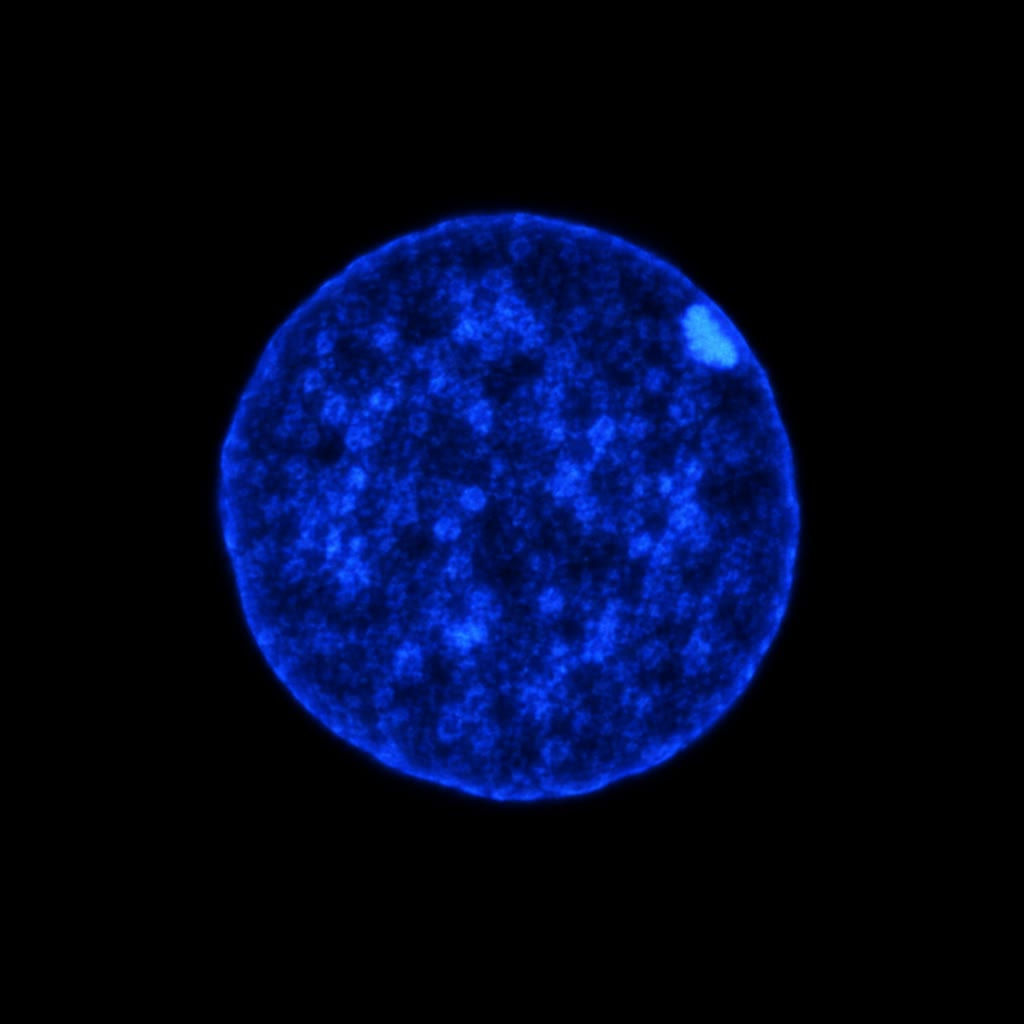
\includegraphics[width=0.42\linewidth]{images/book5/ai/b5-01-barr-body.jpg}\hspace{0.04\linewidth}
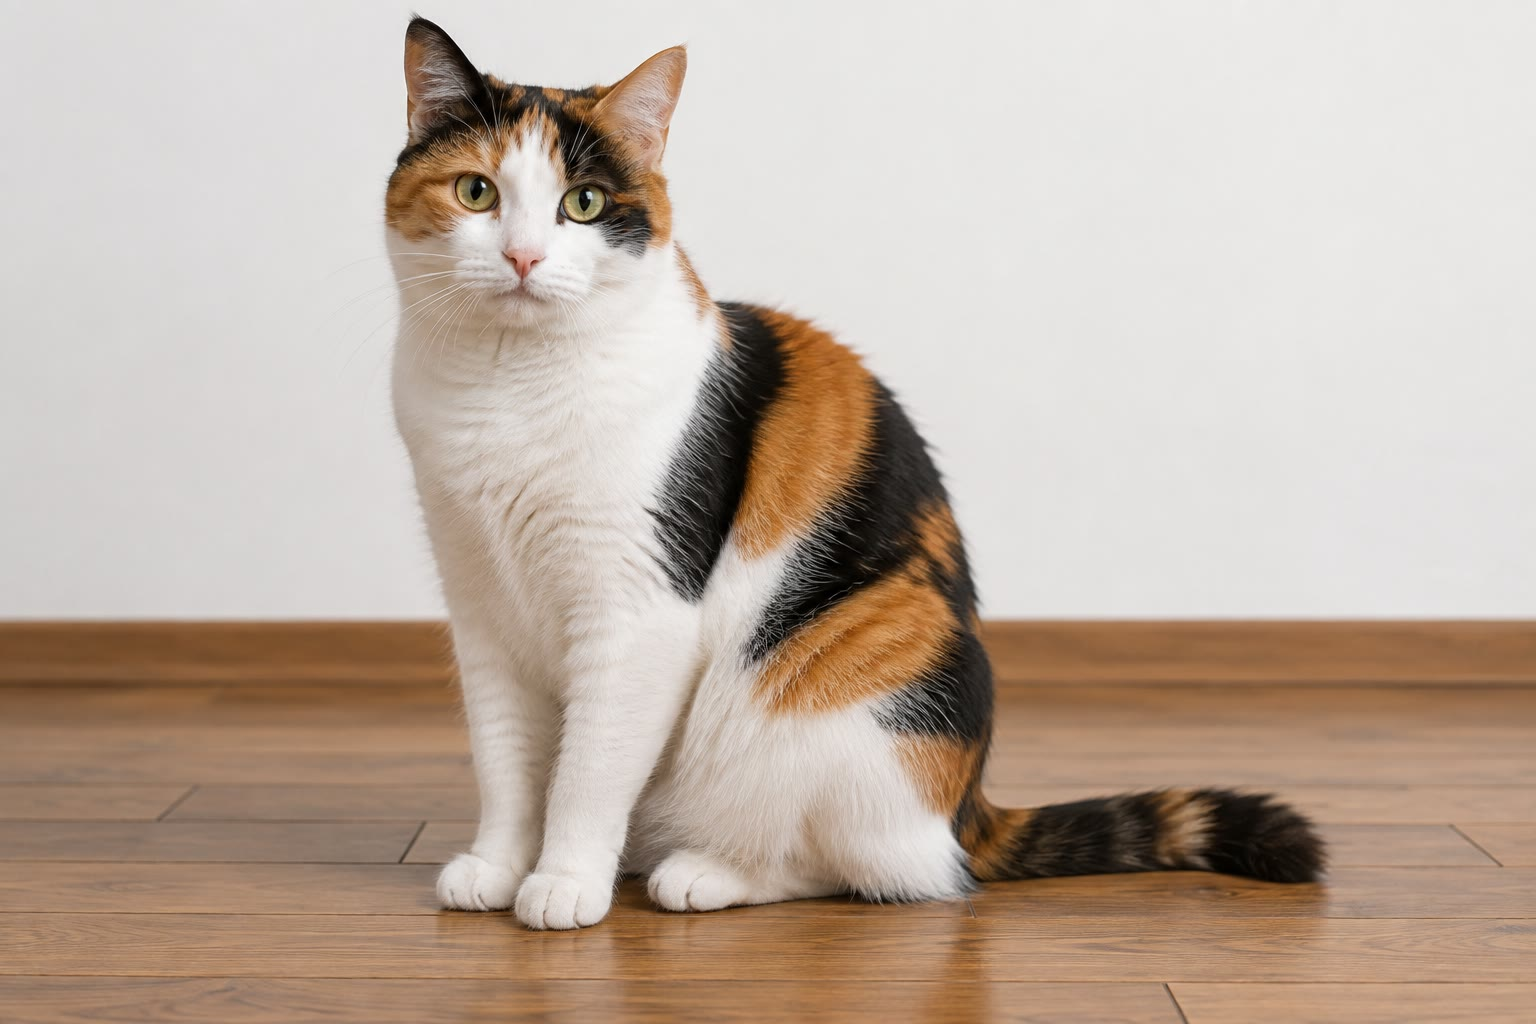
\includegraphics[width=0.5\linewidth]{images/book5/ai/b5-01-calico-cat.jpg}

{\small Links: een vrouwelijke kern gekleurd voor DNA, met de compacte
inactieve X --- het \omterm{def:b3:chromatin-epigenetics:x-inactivation}{Barr-lichaampje} --- tegen de kernrand gedrukt.
Rechts: een lapjeskat. Elke oranje of zwarte plek is een kloon van
huidcellen die hetzelfde X-chromosoom hebben uitgeschakeld; het wit is
een apart, autosomaal, vlekkengen.}
\end{omfigure}

\begin{definition}[Genomische imprinting]\label{def:b3:chromatin-epigenetics:imprinting}
\index{genomische imprinting}\index{imprintingcontroleregio}\index{uniparentale disomie}
Een gen is \emph{geïmprint} wanneer maar één van zijn twee allelen tot
expressie komt, en welk allel dat is hangt af van de ouder waarvan het
komt: sommige genen komen alleen van de vaderlijke kopie tot
expressie, andere alleen van de moederlijke. Zoogdieren hebben zo'n
\numrange{100}{200} geïmprinte genen, in clusters, en elk cluster
wordt bestuurd door een \emph{imprintingcontroleregio} (ICR) die op
het ene ouderlijke allel gemethyleerd is en op het andere niet. De
methylering wordt in de kiembaan ingesteld --- één patroon in
zaadcellen, een ander in eicellen --- in de kiemcellen van de volgende
generatie gewist en opnieuw ingesteld naar het geslacht van dat
individu. Een kind dat beide kopieën van een chromosoom van dezelfde
ouder krijgt (\emph{uniparentale disomie}) heeft daarom de verkeerde
dosis van de geïmprinte genen erop, hoewel zijn sequentie volkomen
normaal is.
\end{definition}

\begin{proof}[Bewijsmateriaal]
McGrath en Solter, en onafhankelijk Surani, Barton en Norris (1984),
maakten muizenzygoten met twee moederlijke voorkernen, of twee
vaderlijke, door voorkernen tussen bevruchte eicellen over te brengen.
Geen van beide soorten kwam tot ontwikkeling, hoewel elk twee
volledige chromosoomsets had: de gynogenetische embryo's vormden een
redelijk embryo met een slechte placenta, de androgenetische een grote
placenta en vrijwel geen embryo. De twee ouderlijke genomen zijn niet
gelijkwaardig en beide zijn nodig. Cattanach en Kirk (1985) toonden
met chromosoomspecifieke uniparentale disomieën aan dat de
ongelijkwaardigheid beperkt is tot bepaalde gebieden van bepaalde
chromosomen, en daar zijn de geïmprinte clusters later gevonden.
\end{proof}

\begin{example}[Het cluster \emph{Igf2}--\emph{H19}]\label{ex:b3:chromatin-epigenetics:igf2}
\emph{Igf2}, een foetale groeifactor, komt tot expressie vanaf het
vaderlijke allel; zijn buurman \emph{H19}, een niet-coderend RNA,
vanaf het moederlijke. Daartussen ligt de ICR en, voorbij \emph{H19},
een gedeelde reeks enhancers. Op het moederlijke chromosoom is de ICR
ongemethyleerd en bindt zij CTCF, dat als isolator werkt: de enhancers
kunnen \emph{H19} bereiken maar \emph{Igf2} niet. Op het vaderlijke
chromosoom is de ICR gemethyleerd (ingesteld in de zaadcel), kan CTCF
niet binden en reiken de enhancers over naar \emph{Igf2}; de
methylering breidt zich ook uit en legt de \emph{H19}-promotor stil.
Eén merkteken, ingesteld in één kiembaan, beslist over beide genen.
\end{example}

\begin{omfigure}
\begin{tikzpicture}[every node/.style={font=\scriptsize}, >=stealth]
  \foreach \yy/\lab/\ctcf in {1.6/moederlijk chromosoom/1, -0.6/vaderlijk chromosoom/0} {
    \draw[very thick, gray] (0,\yy) -- (9.4,\yy);
    \node[left, align=right] at (-0.15,\yy) {\lab};
    \draw[thick, fill=omDef!25] (1.0,\yy-0.2) rectangle (2.6,\yy+0.2); \node at (1.8,\yy) {\emph{Igf2}};
    \draw[thick, fill=omProp!30] (4.2,\yy-0.2) rectangle (5.2,\yy+0.2); \node at (4.7,\yy) {ICR};
    \draw[thick, fill=omDef!25] (6.2,\yy-0.2) rectangle (7.4,\yy+0.2); \node at (6.8,\yy) {\emph{H19}};
    \foreach \x in {8.4,8.8,9.2} \fill[omMeth!70!black] (\x,\yy) circle (0.12);
    \node[right] at (9.55,\yy) {enhancers};
  }
  % maternal: CTCF bound, enhancer -> H19
  \draw[thick, fill=omExo!35] (4.7,2.15) ellipse (0.45 and 0.22); \node at (4.7,2.15) {CTCF};
  \draw[->, thick, omMeth!70!black] (8.4,1.85) .. controls (7.8,2.5) and (7.2,2.5) .. (6.8,1.85);
  \node[above] at (7.6,2.35) {aan};
  \draw[thick, omThm] (5.3,2.3) -- (5.3,0.9); \node[omThm, below] at (5.3,0.9) {isolator};
  \node[omThm, above=1.0cm, align=center, font=\scriptsize] at (1.8,1.8) {\emph{Igf2} zwijgt};
  % paternal: ICR methylated
  \foreach \x in {4.35,4.6,4.85,5.1} \fill[omThm] (\x,-0.95) circle (0.08);
  \node[below, align=center] at (4.7,-1.05) {gemethyleerd:\\geen CTCF};
  \draw[->, thick, omMeth!70!black] (8.4,-0.35) .. controls (6.5,0.6) and (3.5,0.6) .. (1.8,-0.35);
  \node[above] at (3.3,0.2) {aan};
  \foreach \x in {6.4,6.7,7.0,7.2} \fill[omThm] (\x,-0.95) circle (0.08);
  \node[below] at (6.8,-1.05) {uitgeschakeld};
\end{tikzpicture}

{\small Imprinting bij \emph{Igf2}--\emph{H19}. Moederlijk allel: de
ongemethyleerde ICR bindt CTCF, een isolator, zodat de
stroomafwaartse enhancers alleen \emph{H19} activeren. Vaderlijk
allel: de ICR werd in de zaadcel gemethyleerd, CTCF kan niet binden,
de enhancers bereiken \emph{Igf2}, en de methylering legt \emph{H19} stil.}
\end{omfigure}

\begin{example}[Prader--Willi en Angelman]\label{ex:b3:chromatin-epigenetics:pws}
Dezelfde deletie van ongeveer \qty{5}{Mb} in chromosoom 15 (regio
15q11--q13) veroorzaakt het \emph{syndroom van Prader--Willi} ---
slappe spieren bij de geboorte, daarna onverzadigbare eetlust en
obesitas --- wanneer zij op het vaderlijke chromosoom ligt, en het
\emph{syndroom van Angelman} --- ernstige verstandelijke beperking,
afwezige spraak, een vrolijk voorkomen en epilepsie --- wanneer zij op
het moederlijke ligt. De regio draagt vaderlijk tot expressie komende
genen (\emph{SNRPN} en een cluster kleine RNA's) waarvan in het eerste
geval de enige actieve kopie verloren gaat, en het moederlijk tot
expressie komende \emph{UBE3A}, dat in het tweede geval verloren gaat.
Moederlijke \omterm{def:b3:chromatin-epigenetics:imprinting}{uniparentale disomie} van 15, zonder enige deletie, geeft
eveneens Prader--Willi: twee moederlijke kopieën, zwijgend voor de
vaderlijke genen.
\end{example}

\begin{remark}[Waarom eigenlijk imprinten]\label{rem:b3:chromatin-epigenetics:kinship}
Geïmprinte genen zijn verrijkt voor de sturing van de foetale groei en
van het transport van voedingsstoffen door de placenta, waarbij
vaderlijk tot expressie komende genen (\emph{Igf2}, \emph{Peg3})
eerder groei bevorderen en moederlijk tot expressie komende
(\emph{H19}, \emph{Igf2r}, \emph{Cdkn1c}) haar eerder beteugelen. De
\emph{verwantschapstheorie} leest hierin een conflict: de genen van
een vader winnen bij het onttrekken van meer aan een moeder die later
nakomelingen van andere mannetjes kan dragen, terwijl de genen van de
moeder winnen bij het rantsoeneren over al haar worpen. Imprinting
komt voor bij placentadieren en bij bloemplanten, waarvan het
endosperm eveneens door de moeder wordt gevoed, en niet bij vogels of
reptielen, en dat is wat de theorie voorspelt.
\end{remark}

\section{Epigenetische overerving en haar grenzen}

\begin{definition}[Epigenetica]\label{def:b3:chromatin-epigenetics:epigenetics}
\index{epigenetica}\index{epiallel}\index{herprogrammering}
\emph{Epigenetica} is de studie van erfelijke veranderingen in
genactiviteit die geen veranderingen in de DNA-sequentie zijn:
toestanden gedragen door \omterm{def:b3:chromatin-epigenetics:methylation}{DNA-methylering}, histonmerktekens of
zelfonderhoudende circuits van transcriptiefactoren, en gekopieerd
door de celdeling heen. Twee allelen van identieke sequentie maar met
een verschillende stabiele epigenetische toestand zijn
\emph{epiallelen}. Overerving door mitose is de regel en is wat een
gedifferentieerde cel gedifferentieerd houdt. Overerving door meiose,
van ouder op nakomeling, is bij zoogdieren de uitzondering, omdat de
merktekens in twee golven van \emph{herprogrammering} worden gewist:
in de primordiale kiemcellen, waar de imprints en het grootste deel
van de methylering worden uitgevlakt en daarna naar geslacht opnieuw
gezet, en nogmaals in de zygote en het vroege embryo, waar het
vaderlijke genoom actief door TET3 wordt gedemethyleerd en het
moederlijke passief, voordat de eigen patronen van het embryo door
DNMT3 worden aangelegd.
\end{definition}

\begin{example}[De levensvatbare gele agoutimuis]\label{ex:b3:chromatin-epigenetics:agouti}
In het $A^{vy}$-allel is een retrotransposon stroomopwaarts van het
vachtkleurgen \emph{agouti} ingevoegd. Waar de promotor van het
transposon ongemethyleerd is, drijft hij \emph{agouti} in elke cel
onophoudelijk aan; de muis is geel, zwaarlijvig en vatbaar voor
diabetes. Waar hij gemethyleerd is, volgt het gen zijn normale
regeling en is de muis bruin (``pseudoagouti''). Genetisch identieke
nestgenoten spreiden zich over het hele spectrum, en een gele moeder
krijgt meer gele jongen dan een bruine: het \omterm{def:b3:chromatin-epigenetics:epigenetics}{epiallel} wordt door de
moederlijke kiembaan onvolledig gewist. Waterland en Jirtle (2003)
gaven drachtige $A^{vy}$-moeders een voeding rijk aan methyldonoren
(foliumzuur, vitamine B\textsubscript{12}, choline, betaïne) en
verschoven de vacht van de jongen naar bruin. Het milieu van de ene
generatie had een merkteken gezet dat de volgende generatie meedroeg.
\end{example}

\begin{omfigure}
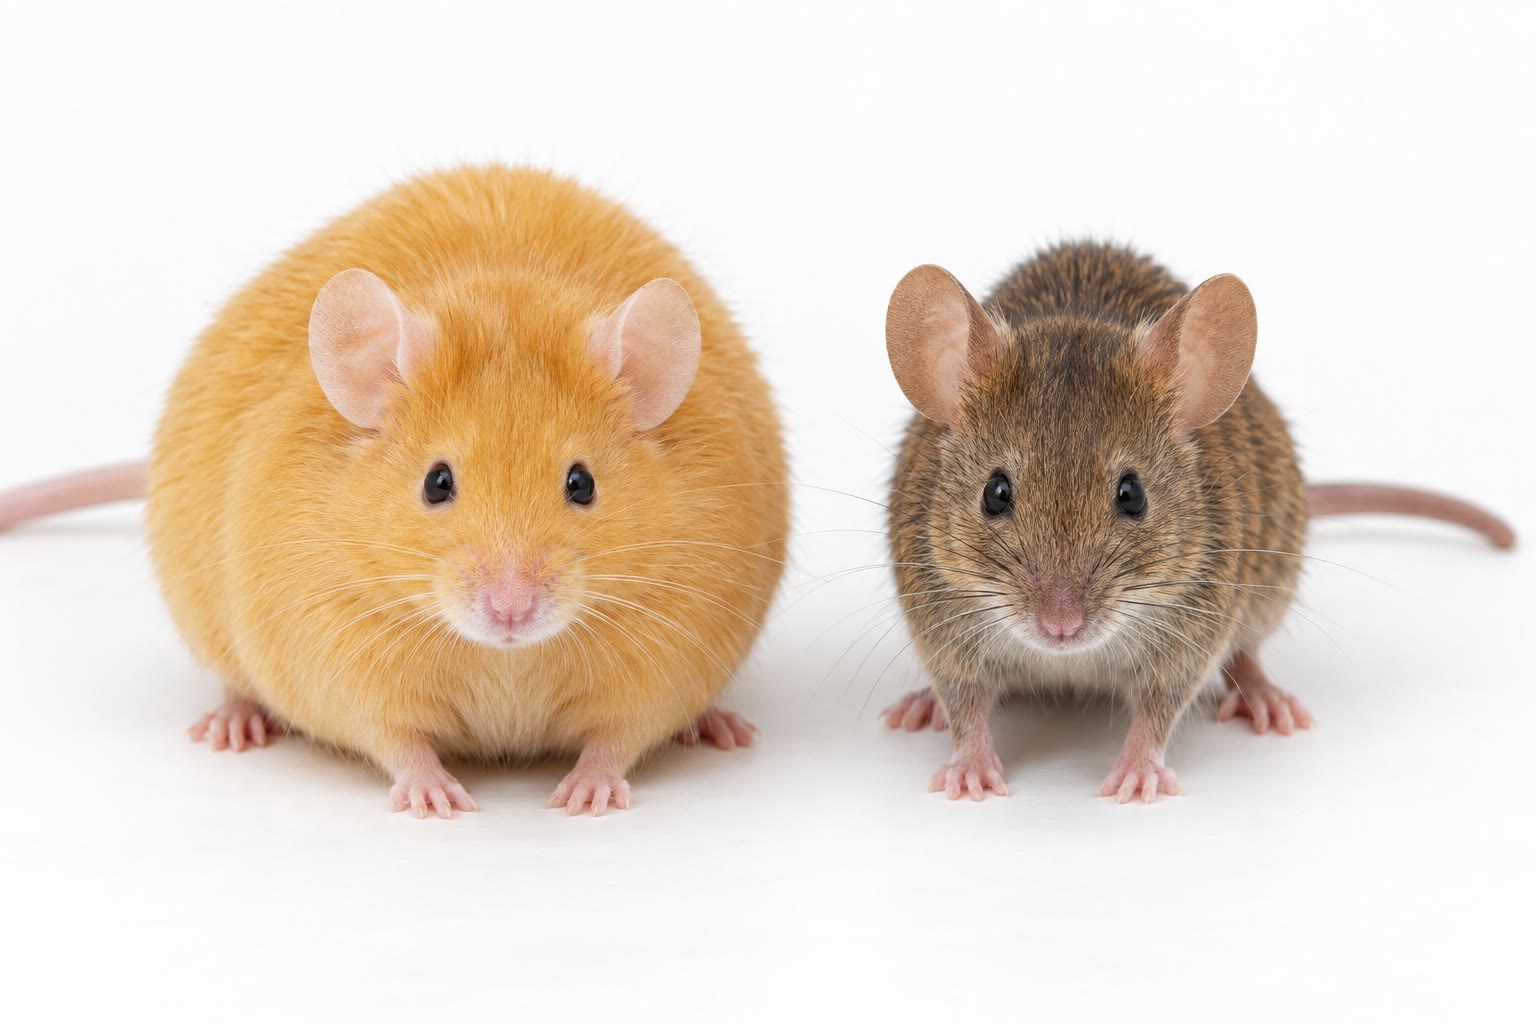
\includegraphics[width=0.62\linewidth]{images/book5/ai/b5-01-agouti-mice.jpg}

{\small Twee $A^{vy}$-nestgenoten met identiek genotype: een gele,
zwaarlijvige muis waarin het transposon stroomopwaarts van
\emph{agouti} ongemethyleerd is, en een bruine pseudoagouti waarin het
gemethyleerd is.}
\end{omfigure}

\begin{proposition}[Waar erfelijke epigenetische toestanden voorkomen]\label{prop:b3:chromatin-epigenetics:examples}
\index{positie-effectvariegatie}\index{vernalisatie}\index{paramutatie}
Drie goed onderzochte systemen illustreren de bovenstaande
mechanismen. \emph{\omterm{prop:b3:chromatin-epigenetics:examples}{Positie-effectvariegatie}} bij \emph{Drosophila}:
een gen dat door een chromosoomherschikking naast \omterm{def:b3:chromatin-epigenetics:nucleosome}{heterochromatine} is
beland, wordt in sommige cellen uitgeschakeld en in andere niet, wat
een gevlamd oog geeft; elke plek is een kloon, de uitschakeling breidt
zich vanuit het \omterm{def:b3:chromatin-epigenetics:nucleosome}{heterochromatine} uit via de HP1-lus, en de genen
waarvan mutatie de variegatie onderdrukt (de \emph{Su(var)}-genen)
zijn HP1 en het H3K9-methyltransferase. \emph{Vernalisatie} bij
\emph{Arabidopsis}: weken winterkou leggen de bloeirepressor
\emph{FLC} stil met door Polycomb neergelegd H3K27me3, de stilte houdt
maanden voorjaarsgroei en duizenden celdelingen stand, en zij wordt in
elke generatie teruggezet, zodat elke plant haar eigen winter moet
meemaken. \emph{Paramutatie} bij mais: één allel van het pigmentgen
\emph{b1} zet, wanneer het in een heterozygoot een bepaald ander allel
ontmoet, dat allel om naar zijn eigen zwijgende toestand, en het
omgezette allel geeft die toestand generaties lang aan zijn
nakomelingen door, via een door klein RNA gestuurde methylering die in
\cref{ch:b3:rna-regulation} aan bod komt. In alle drie de gevallen is
de overerving mitotisch en robuust; de overdracht tussen generaties
wordt ofwel actief teruggezet (planten) ofwel is lek en onvolledig
(muizen).
\end{proposition}

\begin{remark}[De grenzen van transgenerationele claims]\label{rem:b3:chromatin-epigenetics:limits}
Beweringen dat de hongersnood of de stress van een grootouder
``epigenetisch geërfd'' wordt door menselijke kleinkinderen zijn
gangbaar en meestal onbewezen. Tussen een somatisch merkteken en een
kleinkind staan twee golven van uitwissing, de geïmprinte genen en
enkele transposons zijn bij zoogdieren de enige gedocumenteerde
overlevenden van die uitwissing, en in menselijke cohorten zijn de
effecten van een gedeeld milieu, van het milieu in de baarmoeder en
van genetische verschillen moeilijk te scheiden van een merkteken dat
in de kiembaan wordt meegedragen. De aangetoonde gevallen ---
$A^{vy}$, enkele aan transposons gekoppelde \omterm{def:b3:chromatin-epigenetics:epigenetics}{epiallelen}, door RNA
bemiddelde toestanden bij wormen en planten --- zijn echt, moleculair
begrepen en beperkt. De stelling van dit hoofdstuk zegt waarom: zonder
een terugkoppeling die $\mu$ naar $1$ duwt, vergeet een merkteken
zichzelf in enkele tientallen delingen, en de kiembaan legt daar nog
een actieve terugzetting bovenop.
\end{remark}

\section{Opgaven}

\begin{exercise}[$\star$]\label{exo:b3:chromatin-epigenetics:1}
Geef de samenstelling van een nucleosoomkerndeeltje, de lengte van het
DNA dat het bindt en de gebruikelijke linkerlengte. Waarom gaf
nucleasevertering van \omterm{def:b3:chromatin-epigenetics:nucleosome}{chromatine} een ladder van fragmenten en geen
veeg?
\end{exercise}

\begin{exercise}[$\star$]\label{exo:b3:chromatin-epigenetics:2}
Een kikkergenoom heeft $3.0\times 10^{9}$ basenparen per haploïde set.
Hoeveel \omterm{def:b3:chromatin-epigenetics:nucleosome}{nucleosomen} bevat een diploïde kern, uitgaande van een
herhaling van \qty{190}{bp}, en hoe lang is haar DNA?
\end{exercise}

\begin{exercise}[$\star$]\label{exo:b3:chromatin-epigenetics:3}
Ontcijfer H3K27me3, H4K16ac en H3S10ph. Zeg bij elk of het met actief
dan wel met zwijgend \omterm{def:b3:chromatin-epigenetics:nucleosome}{chromatine} samengaat, en noem een \omterm{def:b3:chromatin-epigenetics:histone-code}{lezer} voor het
eerste.
\end{exercise}

\begin{exercise}[$\star$]\label{exo:b3:chromatin-epigenetics:4}
Leg uit waarom een lapjeskat vrijwel altijd vrouwelijk is, en wat een
mannelijke lapjeskat wel moet zijn.
\end{exercise}

\begin{exercise}[$\star\star$]\label{exo:b3:chromatin-epigenetics:5}
Bereken de \omterm{prop:b3:chromatin-epigenetics:compaction}{pakkingsgraad} van de \qty{10}{nm}-vezel uit de getallen van
\cref{def:b3:chromatin-epigenetics:nucleosome} (herhaling
\qty{200}{bp}, kraal \qty{11}{nm}), en de graad die nodig is om de
\qty{4}{cm} DNA van een gemiddeld menselijk chromosoom in een mitotisch
chromatide van \qty{4}{\micro m} te persen. Met welke extra factor moet
de vezel worden gevouwen?
\end{exercise}

\begin{exercise}[$\star\star$]\label{exo:b3:chromatin-epigenetics:6}
Bepaal in het model van \cref{thm:b3:chromatin-epigenetics:maintenance}
met $\mu = 0.98$ en $\delta = 0.01$ de waarde van $p^{*}$ en het aantal
delingen waarna een plaats die gemethyleerd begon de helft van haar
overschot boven $p^{*}$ kwijt is. Herhaal dit voor $\mu = 0.999$,
$\delta = 0.001$.
\end{exercise}

\begin{exercise}[$\star\star$]\label{exo:b3:chromatin-epigenetics:7}
Een ChIP-seq-experiment op levercellen geeft een H3K4me3-piek en een
H3K27ac-piek bij de promotor van gen $A$, een breed H3K27me3-domein
over gen $B$ en H3K9me3 over gen $C$. Voorspel de transcriptionele
toestand van elk, en zeg welke van $B$ en $C$ in een ander celtype
eerder aangezet zal worden, en waarom.
\end{exercise}

\begin{exercise}[$\star\star$]\label{exo:b3:chromatin-epigenetics:8}
Een vrouw draagt op één chromosoom 15 een deletie van de
\emph{UBE3A}-regio maar is gezond. Haar vader droeg dezelfde deletie
en was eveneens gezond. Op welk syndroom loopt elk van haar kinderen
risico, en met welke kans? En als de deletie van haar moeder was
gekomen?
\end{exercise}

\begin{exercise}[$\star\star$]\label{exo:b3:chromatin-epigenetics:9}
Voorspel wat er in een vrouwelijk muizenembryo gebeurt als het
\emph{\omterm{def:b3:chromatin-epigenetics:x-inactivation}{Xist}}-gen van één X-chromosoom wordt verwijderd; en van beide.
Voorspel wat een \emph{\omterm{def:b3:chromatin-epigenetics:x-inactivation}{Xist}}-transgen dat in een autosoom is ingebouwd
met dat autosoom doet.
\end{exercise}

\begin{exercise}[$\star\star\star$]\label{exo:b3:chromatin-epigenetics:10}
Leg met \cref{ex:b3:chromatin-epigenetics:cpg-deficit} uit waarom
\omterm{def:b3:chromatin-epigenetics:methylation}{CpG-eilanden} hun \omterm{def:b3:chromatin-epigenetics:methylation}{CpG}'s hebben behouden terwijl de rest van het genoom
er vier vijfde van heeft verloren, en wat dit zegt over de
methyleringstoestand van de eilanden in de kiembaan op evolutionaire
tijdschaal. Waarom gaat het argument niet op voor een gen dat alleen
in de lever gemethyleerd is?
\end{exercise}

\begin{exercise}[$\star\star\star$]\label{exo:b3:chromatin-epigenetics:11}
Laat met de lus van \omterm{def:b3:chromatin-epigenetics:histone-code}{schrijver} en \omterm{def:b3:chromatin-epigenetics:histone-code}{lezer} uit
\cref{prop:b3:chromatin-epigenetics:readers} zien hoe een domein van
H3K9me3 stabiel kan blijven door de replicatie heen, hoewel elke
deling de gemerkte \omterm{def:b3:chromatin-epigenetics:nucleosome}{histonen} tweevoudig verdunt met nieuwe ongemerkte.
Wat bepaalt waar het domein ophoudt zich uit te breiden? Stel een
experiment voor om die verklaring te toetsen.
\end{exercise}

\begin{exercise}[$\star\star\star$]\label{exo:b3:chromatin-epigenetics:12}
Een studie meldt dat de kleinkinderen van mensen die een hongersnood
hebben meegemaakt een afwijkende methylering bij een groeigen en een
hogere lichaamsmassa hebben. Noem de alternatieve verklaringen die
moeten worden uitgesloten voordat men mag besluiten dat een
methyleringsmerkteken via de kiembaan is doorgegeven, en zeg welk
experiment bij muizen de vraag zou beslechten.
\end{exercise}

\section{Vraagstuk: het geheugen van een uitgeschakeld gen}

\begin{problem}[{Weekendvraagstuk --- een menselijk genoom gepakt in zijn
kern, een methyleringsmerkteken gevolgd door de delingen heen, een
lapjeskat gelezen als een klonale kaart en de ziekten van een
geïmprinte regio geteld, met als besluit het aantal delingen dat een
merkteken zonder terugkoppeling overleeft en de grootte van de
celpopulatie die haar X koos}]
\label{pb:b3:chromatin-epigenetics:1}
Gegevens: een menselijke diploïde kern bevat $6.4\times 10^{9}$
basenparen, à \qty{0.34}{nm} en \qty{650}{Da} per paar; de
nucleosoomherhaling is \qty{200}{bp}, een histonoctameer weegt
\qty{108}{kDa}, en een kerndeeltje is een schijf van \qty{11}{nm}
doorsnede en \qty{5.5}{nm} dik. De kern is een bol met diameter
\qty{10}{\micro m}. Het genoom is voor \qty{42}{\%} G$+$C. Methylering
op een gewoon \omterm{def:b3:chromatin-epigenetics:methylation}{CpG}: $\mu = 0.99$, $\delta = 0.02$ per deling.

\medskip
\noindent\textbf{Deel I --- Pakking.}
\begin{enumerate}
  \item Bereken de totale lengte van het DNA in de kern en het aantal
        \omterm{def:b3:chromatin-epigenetics:nucleosome}{nucleosomen}.
  \item Bereken de totale massa aan \omterm{def:b3:chromatin-epigenetics:nucleosome}{histon} (alleen octameren) en aan
        DNA, in picogram ($\qty{1}{Da} = \qty{1.66e-24}{g}$).
  \item Bereken het volume van de kern en het totale volume van de
        kerndeeltjes, opgevat als cilinders. Welk deel van de kern
        vullen zij?
  \item Als de \omterm{def:b3:chromatin-epigenetics:nucleosome}{nucleosomen} als een \qty{10}{nm}-vezel achter elkaar
        zouden liggen, hoe lang zou die vezel dan zijn, en wat is de
        \omterm{prop:b3:chromatin-epigenetics:compaction}{pakkingsgraad} ten opzichte van naakt DNA?
  \item De vezel is gevouwen tot lussen van \qty{200}{kb} verankerd
        door cohesine. Hoeveel lussen, en hoeveel \omterm{def:b3:chromatin-epigenetics:nucleosome}{nucleosomen} per lus?
  \item Hoeveel CpG-dinucleotiden zou het diploïde genoom onder de
        aanname van onafhankelijkheid bevatten? Het waargenomen aantal
        is $5.6\times 10^{7}$. Welk deel is verloren gegaan, en door
        welk mutatiemechanisme?
\end{enumerate}

\medskip
\noindent\textbf{Deel II --- Een merkteken door de delingen heen.}
\begin{enumerate}[resume]
  \item Schrijf de recursie voor $p_{n}$ op en bereken $p^{*}$.
  \item Een \omterm{def:b3:chromatin-epigenetics:methylation}{promotor-CpG} is bij $n = 0$ volledig gemethyleerd. Bereken
        $p_{n}$ na $10$, $50$ en $200$ delingen.
  \item Na hoeveel delingen is het overschot $p_{n} - p^{*}$ gehalveerd?
        Een weefselstamcel deelt ongeveer eens per week: hoeveel jaar
        is dat?
  \item Een geneesmiddel remt \omterm{def:b3:chromatin-epigenetics:methylation}{DNMT1} volledig ($\mu = 0$) en DNMT3
        eveneens ($\delta = 0$). Laat zien dat de fractie gemethyleerde
        strengen in de populatie bij elke deling halveert, en bepaal
        het aantal delingen om \qty{80}{\%} methylering onder
        \qty{5}{\%} te brengen.
  \item In een uitgeschakeld eiland trekken de methyl-CpG-lezers
        H3K9-methylering aan, die DNMT3 aantrekt, zodat binnen het
        eiland $\mu = 0.9995$ en $\delta = 0.0005$. Herbereken de
        halveringstijd van het overschot, in delingen en in jaren bij
        één deling per week.
  \item Leg in één zin uit waarom de uitkomst van vraag 11 en niet die
        van vraag 9 is wat een levenslang uitgeschakeld gen vereist, en
        welke moleculaire opstelling haar voortbrengt.
\end{enumerate}

\medskip
\noindent\textbf{Deel III --- De kaart van de lapjeskat.}
\begin{enumerate}[resume]
  \item Een kat is heterozygoot voor het X-gebonden oranjegen. Leg uit
        waarom haar vacht oranje en zwarte plekken heeft en wat één
        plek voorstelt.
  \item De \omterm{def:b3:chromatin-epigenetics:x-inactivation}{X-inactivatie} vond plaats toen de cellen die de huid zouden
        vormen met $N$ waren. Elk koos willekeurig een X. Wat is de
        kans dat alle $N$ dezelfde kozen, wat een eenkleurige kat zou
        geven?
  \item Onder misschien een miljard katten is zo'n eenkleurige
        heterozygoot nooit beschreven; neem de kans op $10^{-9}$ en
        schat $N$.
  \item Het huidoppervlak van de kat is ongeveer \qty{0.3}{m^2} en haar
        plekken zijn gemiddeld \qty{15}{cm^2}. Schat het aantal
        plekken, en leg uit waarom het groter is dan $N$.
  \item Een XXY-kater is ook een lapjeskat. Hoeveel \omterm{def:b3:chromatin-epigenetics:x-inactivation}{Barr-lichaampjes}
        tonen zijn cellen? Hoeveel bij een XXX-vrouwtje en bij een
        XY-mannetje?
  \item Een gen dat aan de inactivatie ontsnapt is bij vrouwtjes in
        twee actieve kopieën aanwezig en bij mannetjes in één. Geef één
        reden waarom zulke ontsnapping verdragen kan worden en één
        situatie waarin zij ertoe doet.
\end{enumerate}

\medskip
\noindent\textbf{Deel IV --- Chromosoom 15.}
\begin{enumerate}[resume]
  \item Het syndroom van Prader--Willi treft ongeveer één geboorte op
        \num{15000}; \qty{70}{\%} van de gevallen is een de-novodeletie
        van het vaderlijke 15q11--q13 en \qty{25}{\%} een moederlijke
        \omterm{def:b3:chromatin-epigenetics:imprinting}{uniparentale disomie}. Bereken de geboortefrequentie van elke
        oorzaak.
  \item Het syndroom van Angelman heeft ongeveer dezelfde frequentie;
        \qty{70}{\%} zijn moederlijke deleties, \qty{5}{\%} vaderlijke
        disomieën en \qty{10}{\%} puntmutaties van \emph{UBE3A}. Waarom
        zijn puntmutaties wel een oorzaak van Angelman maar vrijwel
        nooit van Prader--Willi?
  \item Een vader draagt een gebalanceerde translocatie die
        \qty{20}{\%} van zijn zaadcellen een deletie van 15q11--q13
        geeft. Welk deel van zijn kinderen krijgt Prader--Willi, en
        welk deel Angelman?
  \item \omterm{def:b3:chromatin-epigenetics:imprinting}{Uniparentale disomie} ontstaat wanneer een trisome zygote één
        chromosoom verliest. Als een trisomie-15-zygote willekeurig een
        van haar drie chromosomen verliest, en de trisomie van de
        moeder kwam (twee moederlijke kopieën), wat is dan de kans dat
        de overlevende moederlijke disomie heeft? Welk syndroom?
  \item De Prader--Willi-genen komen vaderlijk tot expressie en het
        Angelman-gen moederlijk. Zeg met de verwantschapstheorie welke
        van de symptomen van de twee syndromen (voedingsproblemen bij
        de geboorte tegenover vraatzucht) bij de theorie passen en
        welke moeilijker te plaatsen zijn.
  \item Er wordt een methode voorgesteld om Angelman te behandelen door
        het zwijgende vaderlijke \emph{UBE3A} weer aan te zetten. Zijn
        stilte komt door een vaderlijk tot expressie komend
        antisense-RNA. Stel het moleculaire doelwit voor en zeg waarom
        de therapie de andere geïmprinte genen niet zou verstoren.
  \item Vat samen: de halveringstijd van een merkteken zonder
        terugkoppeling (vraag~9) en met terugkoppeling (vraag~11), in
        delingen; en de stichterspopulatie $N$ van de lapjesvacht
        (vraag~15).
\end{enumerate}
\end{problem}
